\documentclass[conference,onecolumn,10pt]{IEEEtran}
\usepackage[utf8]{inputenc}
\usepackage[T1]{fontenc}
\usepackage{lmodern}
\usepackage{graphicx}
\usepackage{booktabs}
\usepackage{url}
\usepackage{tikz}
\usetikzlibrary{arrows.meta, positioning, calc}
\usepackage{listings}
\usepackage{xcolor}
\usepackage{hyperref}

\lstdefinestyle{p4}{
  basicstyle=\ttfamily\footnotesize,
  keywordstyle=\color{blue!70!black}\bfseries,
  commentstyle=\color{green!45!black}\itshape,
  stringstyle=\color{red!60!black},
  morekeywords={table,action,key,actions,apply,control,header,struct,
    lpm,exact,default_action,size,bit,counter,register,direct_counter},
  comment=[l]{//},
  showstringspaces=false,
  columns=fullflexible,
  keepspaces=true,
  frame=single,
  framesep=4pt,
  aboveskip=6pt, belowskip=4pt,
}

\begin{document}

\title{Redes Programables y el Lenguaje P4:\\
Del Plano de Datos Fijo al Plano de Datos Programable}

\author{
\IEEEauthorblockN{Christopher Zúñiga (C28730) \quad Adrian Hernandez (C39321)}
\IEEEauthorblockA{Curso de Redes de Computadoras\\
Investigación \#2 --- Redes Programables con P4\\
Junio de 2026\\
Repositorio: \url{https://github.com/czuniga28/redes-programables-p4}}
}

\maketitle

\begin{abstract}
Las redes tradicionales se construyeron sobre dispositivos cuyo plano de datos
era fijo: el conjunto de protocolos y operaciones que un switch o router podía
ejecutar venía determinado por el fabricante en silicio. Este modelo limitó la
velocidad de innovación y obligó a los operadores a esperar ciclos de hardware
de años para soportar nuevos encabezados o funciones. El surgimiento del plano
de datos programable, y en particular del lenguaje P4 (\emph{Programming
Protocol-Independent Packet Processors}), invirtió esta relación: el ingeniero
define cómo se parsea, procesa y reenvía cada paquete, y compila ese
comportamiento hacia objetivos de software (BMv2), ASIC (Tofino) o FPGA. Este
informe revisa la evolución del plano de datos, la arquitectura y el modelo de
ejecución de P4 (PISA), el protocolo P4Runtime para la comunicación con el plano
de control vía gRPC, y casos de uso representativos como la telemetría in-band
(INT), el balanceo de carga programable y las funciones de seguridad en el plano
de datos, incluyendo despliegues de producción en hiperescaladores.
\end{abstract}

\begin{IEEEkeywords}
Redes programables, P4, SDN, plano de datos, PISA, P4Runtime, BMv2, INT.
\end{IEEEkeywords}

\section{Introducción}
Durante décadas, la arquitectura de los equipos de red siguió un patrón
\emph{bottom-up}: el hardware fijaba qué protocolos existían y el software de
control se adaptaba a esas capacidades. Un switch Ethernet ``sabía'' procesar
VLAN, IPv4 o MPLS porque su circuito integrado de aplicación específica (ASIC)
había sido diseñado para ello. Añadir un nuevo encabezado —por ejemplo, un
formato de encapsulamiento para centros de datos— implicaba un nuevo \emph{tape
out} de silicio, un proceso de varios años y altísimo costo
\cite{bosshart2013rmt}.

La programabilidad del plano de datos propone el patrón inverso, \emph{top-down}:
el operador describe en un lenguaje de alto nivel cómo deben tratarse los
paquetes, y un compilador traduce esa descripción a una pipeline configurable.
P4 es hoy el lenguaje de facto para expresar ese comportamiento
\cite{bosshart2014p4}. Este trabajo construye el marco conceptual necesario para
comprender la arquitectura del plano de datos programable, como base para las
implementaciones de laboratorio (un router IPv4 estático y un sistema de
contadores de tráfico) que acompañan a esta investigación.

\section{Evolución del Plano de Datos}

\subsection{Limitaciones del modelo de red tradicional}
En el modelo clásico, el plano de datos es \emph{fixed-function}: el conjunto de
campos reconocibles, las tablas de coincidencia y las acciones disponibles están
cableados. Esto acarrea tres limitaciones fundamentales:

\begin{itemize}
\item \textbf{Rigidez de protocolos.} Soportar un nuevo encabezado requiere
hardware nuevo. Los operadores quedan atados al catálogo de protocolos que el
fabricante decidió implementar.
\item \textbf{Innovación lenta.} El ciclo de diseño de un ASIC de red ronda los
2--3 años, lo que desacopla la velocidad de la investigación de redes de la
velocidad del despliegue real \cite{bosshart2013rmt}.
\item \textbf{Opacidad y dependencia del proveedor.} El comportamiento exacto del
\emph{forwarding} es una caja negra; el operador no puede auditar ni modificar
cómo se procesa internamente un paquete.
\end{itemize}

\subsection{Surgimiento del plano de datos programable}
Dos avances habilitaron el cambio. Primero, la \emph{Software-Defined
Networking} (SDN) separó el plano de control del plano de datos, centralizando
la lógica de decisión en un controlador \cite{mckeown2008openflow}. Segundo, el
trabajo sobre \emph{Reconfigurable Match Tables} (RMT) demostró que era posible
construir un ASIC con una pipeline de \emph{match-action} reconfigurable a
velocidad de línea (terabits por segundo) sin sacrificar rendimiento
\cite{bosshart2013rmt}. RMT probó que ``programable'' y ``rápido'' no eran
mutuamente excluyentes, abriendo la puerta a que el plano de datos —no solo el de
control— fuera definido por software.

\subsection{SDN clásica (OpenFlow) frente a P4}
OpenFlow fue el primer protocolo SDN ampliamente adoptado, pero opera sobre un
plano de datos \emph{fijo}: define un conjunto cerrado y creciente de campos de
coincidencia (\emph{match fields}) que el switch debe entender de antemano. Cada
nueva versión de OpenFlow añadía campos (de 12 en la v1.0 a más de 40 en
versiones posteriores), evidenciando que un enfoque ``enumerar todos los
protocolos posibles'' no escala \cite{bosshart2014p4}.

P4 ataca el problema en la raíz: en lugar de fijar los protocolos, deja que el
programador los \emph{declare}. La Tabla~\ref{tab:openflow-p4} resume las
diferencias.

\begin{table}[t]
\caption{OpenFlow (SDN clásica) vs. P4}
\label{tab:openflow-p4}
\centering
\small
\begin{tabular}{@{}p{2.4cm}p{2.5cm}p{2.6cm}@{}}
\toprule
\textbf{Aspecto} & \textbf{OpenFlow} & \textbf{P4} \\
\midrule
Plano de datos & Fijo (campos predefinidos) & Programable (parser definido por el usuario) \\
Protocolos & Catálogo cerrado, crece por versión & Independiente del protocolo \\
Rol del estándar & Protocolo control--switch & Lenguaje para describir el data plane \\
Pipeline & Tablas con semántica fija & Match-action definidas por el programa \\
Control & Controlador OpenFlow & P4Runtime / gRPC \\
\bottomrule
\end{tabular}
\end{table}

Es importante notar que P4 y SDN no son excluyentes: P4 describe \emph{qué} hace
el switch, mientras que un protocolo de control (P4Runtime) cumple el rol que
OpenFlow tenía de poblar las tablas en tiempo de ejecución.

\section{El Lenguaje P4}

\subsection{Historia y motivación}
P4 fue presentado formalmente por Bosshart \emph{et al.} en 2014 en \emph{ACM
SIGCOMM Computer Communication Review} \cite{bosshart2014p4}. El artículo
planteaba tres objetivos de diseño que siguen vigentes:

\begin{enumerate}
\item \textbf{Reconfigurabilidad}: el controlador debe poder redefinir el
parsing y el procesamiento de paquetes en el campo.
\item \textbf{Independencia de protocolo}: el switch no debe estar atado a
protocolos específicos; estos se describen en el programa.
\item \textbf{Independencia del objetivo (\emph{target})}: el mismo programa debe
poder compilarse a distintos dispositivos sin que el programador conozca los
detalles del hardware.
\end{enumerate}

La motivación surgió directamente de las limitaciones de OpenFlow y del trabajo
RMT: si el hardware ya podía ser reconfigurable, hacía falta un lenguaje de alto
nivel, independiente del fabricante, para expresar esa configuración
\cite{bosshart2014p4, bosshart2013rmt}.

\subsection{Arquitectura de un programa P4}
Un programa P4 (en su versión $P4_{16}$ \cite{p4spec}) se organiza en bloques
funcionales que reflejan el recorrido de un paquete por la pipeline:

\begin{itemize}
\item \textbf{Parsers.} Una máquina de estados que extrae los encabezados del
flujo de bits entrante. Cada estado lee un encabezado y decide la transición
según un campo (p.\,ej., el \texttt{etherType} para pasar de Ethernet a IPv4).
\item \textbf{Match-action tables.} El corazón del modelo. Cada tabla define una
\emph{clave} (campos a coincidir, con semántica \emph{exact}, \emph{lpm} o
\emph{ternary}) y un conjunto de \emph{acciones} posibles. El plano de control
puebla las entradas; el plano de datos, ante cada paquete, busca la entrada
coincidente y ejecuta su acción (p.\,ej., decrementar el TTL y fijar el puerto de
salida).
\item \textbf{Control flows.} La lógica imperativa (bloques \texttt{apply}) que
encadena la aplicación de tablas y condicionales, definiendo el orden del
procesamiento en ingreso y egreso.
\item \textbf{Deparsers.} El proceso inverso al parser: reensambla los
encabezados (posiblemente modificados) de vuelta en un flujo de bits para
transmitir el paquete.
\end{itemize}

En el laboratorio asociado, el router IPv4 ejemplifica este flujo: un parser para
Ethernet/IPv4, una tabla \texttt{ipv4\_lpm} con coincidencia \emph{Longest Prefix
Match}, acciones que reescriben las MAC y decrementan el TTL, y un deparser que
recompone la trama. El Listado~\ref{lst:lpm} muestra, en $P4_{16}$, la
declaración de esa tabla: nótese que el programa describe \emph{qué} campo se
coincide y \emph{qué} acciones existen, pero las entradas concretas las instala
el plano de control.

\begin{lstlisting}[style=p4, caption={Tabla de enrutamiento LPM en P4 (extracto del router del laboratorio).}, label={lst:lpm}]
action ipv4_forward(macAddr_t dstAddr, egressSpec_t port) {
    standard_metadata.egress_spec = port;
    hdr.ethernet.dstAddr = dstAddr;     // MAC del siguiente salto
    hdr.ipv4.ttl = hdr.ipv4.ttl - 1;    // decremento de TTL
}
table ipv4_lpm {
    key     = { hdr.ipv4.dstAddr: lpm; }
    actions = { ipv4_forward; drop; NoAction; }
    size    = 1024;
    default_action = drop();            // sin ruta => descarte
}
\end{lstlisting}

\subsection{Modelo de ejecución PISA}
P4 asume un modelo abstracto de máquina conocido como \emph{PISA} (Protocol
Independent Switch Architecture). En PISA, el paquete atraviesa secuencialmente:
(1) un \emph{parser} programable; (2) una serie de etapas de \emph{match-action}
en el ingreso; (3) un \emph{traffic manager} que encola y replica paquetes; (4)
etapas de match-action en el egreso; y (5) un \emph{deparser}
\cite{bosshart2013rmt, p4spec}. Cada etapa dispone de memoria (TCAM/SRAM) para
tablas y de unidades aritmético-lógicas para las acciones, todo ejecutándose a
velocidad de línea. La clave de PISA es que esta estructura es
\emph{independiente del protocolo}: no hay nada intrínsecamente ``IPv4'' o
``Ethernet'' en el hardware; esos conceptos los introduce el programa P4.

La Fig.~\ref{fig:pisa} esquematiza este recorrido.

\begin{figure}[t]
\centering
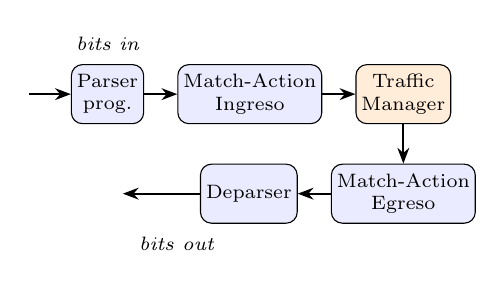
\begin{tikzpicture}[
  node distance=4.2mm,
  box/.style={draw, rounded corners, minimum height=7.5mm, align=center,
    font=\scriptsize, fill=blue!8, inner sep=2pt},
  tm/.style={draw, rounded corners, minimum height=7.5mm, align=center,
    font=\scriptsize, fill=orange!15, inner sep=2pt},
  arr/.style={-{Stealth[length=2mm]}, thick}]
\node[box] (p)  {Parser\\prog.};
\node[box, right=of p] (i) {Match-Action\\Ingreso};
\node[tm,  right=of i] (t) {Traffic\\Manager};
\node[box, below=5mm of t] (e) {Match-Action\\Egreso};
\node[box, left=of e] (d) {Deparser};
\draw[arr] (-1.0,0) -- (p);
\draw[arr] (p) -- (i);
\draw[arr] (i) -- (t);
\draw[arr] (t) -- (e);
\draw[arr] (e) -- (d);
\draw[arr] (d) -- ($(d)-(1.6,0)$);
\node[font=\scriptsize\itshape, above=0.5mm of p] {bits in};
\node[font=\scriptsize\itshape, below left=0.5mm and -3mm of d] {bits out};
\end{tikzpicture}
\caption{Pipeline abstracto PISA: parser programable, etapas de match-action en
ingreso, \emph{traffic manager}, match-action en egreso y deparser. Ninguna
etapa conoce protocolos de antemano; los define el programa P4.}
\label{fig:pisa}
\end{figure}

La arquitectura concreta se expone al programador mediante un \emph{architecture
model}. El más común para aprendizaje es \texttt{v1model} (usado por BMv2), que
define los bloques \texttt{parser}, \texttt{ingress}, \texttt{egress},
\texttt{deparser} y los \emph{externs} disponibles (contadores, registros,
\emph{meters}, funciones de \emph{hash}). Arquitecturas como PSA (Portable Switch
Architecture) o TNA (Tofino Native Architecture) ofrecen modelos más ricos para
hardware real.

\subsection{Tipos de \emph{targets}}
Un mismo programa P4 puede compilarse a objetivos muy distintos:

\begin{itemize}
\item \textbf{BMv2 (software).} El \emph{behavioral model} versión 2 es un switch
P4 de referencia que corre en CPU; no es de alto rendimiento, pero es ideal para
desarrollo, pruebas y docencia \cite{bmv2}. Es el objetivo usado en este
laboratorio junto con Mininet.
\item \textbf{Tofino (ASIC).} La familia Intel/Barefoot Tofino implementa PISA en
silicio y procesa a varios Tbps, siendo el principal objetivo de hardware de
producción para P4 \cite{bosshart2013rmt}.
\item \textbf{FPGAs y SmartNICs.} Plataformas como NetFPGA o las SmartNIC con
soporte P4 permiten desplegar pipelines programables cerca del servidor,
útiles para \emph{offloading} y funciones de red virtualizadas.
\end{itemize}

Esta portabilidad —escribir una vez, compilar a múltiples objetivos— es uno de
los argumentos centrales a favor de P4.

\subsection{Primitivos de estado: contadores, \emph{registers} y \emph{meters}}
Más allá del \emph{forwarding}, P4 expone \emph{externs} que permiten mantener
estado en el plano de datos, esenciales para monitoreo y telemetría. La
Tabla~\ref{tab:state} los compara. Estos primitivos son la base del segundo
laboratorio de esta investigación, que mide tráfico por flujo y por protocolo.

\begin{table}[t]
\caption{Primitivos de estado en P4 ($v1model$)}
\label{tab:state}
\centering
\small
\begin{tabular}{@{}p{1.6cm}p{3.0cm}p{2.7cm}@{}}
\toprule
\textbf{Primitivo} & \textbf{Qué hace} & \textbf{Uso típico} \\
\midrule
\texttt{counter} & Cuenta paquetes y/o bytes en celdas indexadas & Estadísticas por protocolo, por puerto \\
\texttt{direct\_counter} & Contador ligado 1:1 a las entradas de una tabla & Conteo por flujo / por regla \\
\texttt{register} & Memoria de lectura/escritura arbitraria por índice & Estado por flujo, detección de elefantes \\
\texttt{meter} & Marca paquetes según tasa (RFC 2698) & Limitación de tasa, QoS \\
\bottomrule
\end{tabular}
\end{table}

Mientras que un \texttt{counter} solo incrementa, un \texttt{register} permite
\emph{leer-modificar-escribir} dentro del pipeline, habilitando algoritmos con
estado a velocidad de línea (p.\,ej., acumular los bytes de un flujo y compararlos
contra un umbral para marcarlo como ``elefante''). Los \emph{direct counters},
asociados a entradas de tabla, son la forma natural de contabilizar por flujo sin
gestionar índices manualmente. La distinción es importante: P4 no solo decide
\emph{a dónde} va un paquete, sino que puede \emph{recordar} información entre
paquetes, base de la telemetría y la seguridad en el data plane.

\section{P4Runtime y el Plano de Control}

\subsection{Rol del plano de control}
Un programa P4 define la \emph{estructura} del plano de datos (qué tablas
existen, qué acciones soportan), pero no su \emph{contenido}: las entradas
concretas de las tablas las instala el plano de control en tiempo de ejecución.
En el router del laboratorio, por ejemplo, el programa declara la tabla
\texttt{ipv4\_lpm}, pero las rutas estáticas (prefijo $\rightarrow$ siguiente
salto, puerto) las inserta el control plane. Esta separación es la misma idea de
SDN, ahora extendida a un data plane definido por el usuario.

\subsection{P4Runtime y gRPC}
P4Runtime es la API estándar, independiente del objetivo, para que un controlador
gestione un dispositivo P4 en ejecución \cite{p4runtime}. Sus características
principales:

\begin{itemize}
\item Se basa en \textbf{gRPC} y \emph{Protocol Buffers}, lo que le da eficiencia,
\emph{streaming} bidireccional y soporte multiplataforma.
\item Es \textbf{independiente del programa}: el controlador descubre las tablas y
acciones a partir del archivo \texttt{P4Info} que genera el compilador, en lugar
de tener cableados los nombres de campos.
\item Permite insertar/leer entradas de tablas, leer contadores y \emph{registers},
y recibir notificaciones (p.\,ej., paquetes enviados al controlador).
\end{itemize}

En el laboratorio se emplea, como alternativa didáctica, la interfaz
\emph{thrift} de BMv2 (\texttt{simple\_switch\_CLI}) para poblar tablas y leer
contadores; conceptualmente cumple el mismo rol que P4Runtime, aunque este último
es el camino estándar para producción.

\subsection{Comparación con OpenFlow}
P4Runtime y OpenFlow comparten el propósito de comunicar un controlador con el
\emph{forwarding plane}, pero difieren en un punto esencial:

\begin{itemize}
\item \textbf{OpenFlow} asume un pipeline de tablas con semántica fija; el
controlador manipula campos que el protocolo ya conoce.
\item \textbf{P4Runtime} es \emph{agnóstico al esquema}: las tablas, campos y
acciones provienen del programa P4 cargado, descritos en \texttt{P4Info}. Cambiar
el programa P4 cambia automáticamente la ``API'' que ve el controlador, sin
necesidad de un nuevo estándar.
\end{itemize}

Dicho de otro modo, OpenFlow estandariza \emph{el contenido}; P4 + P4Runtime
estandarizan \emph{el mecanismo}, dejando el contenido a cargo del programa
\cite{bosshart2014p4, p4runtime}.

\section{Casos de Uso Relevantes}

\subsection{In-Band Network Telemetry (INT)}
INT es quizá la aplicación insignia de P4. Cada switch programable inserta
metadatos en los propios paquetes de datos a su paso —identificador de switch,
puerto de entrada/salida, tiempo de encolamiento, marca de tiempo—, de modo que
el último salto puede reconstruir la ruta completa y el estado de la red
\emph{sin sondeo activo} \cite{int_spec}. Esto habilita una visibilidad por
paquete imposible en redes tradicionales, útil para detectar microrráfagas y
diagnosticar latencias.

\subsection{Balanceo de carga programable}
P4 permite implementar balanceo de carga directamente en el plano de datos, a
velocidad de línea. Un ejemplo notable es HULA, que mantiene en \emph{registers}
información de congestión por trayecto y selecciona el siguiente salto menos
congestionado, logrando balanceo sensible a la carga sin involucrar al
controlador en cada decisión \cite{katta2016hula}. El laboratorio de contadores
de esta investigación usa los mismos primitivos (\emph{registers}, contadores)
que sustentan estas técnicas.

\subsection{Funciones de seguridad en el plano de datos}
Al poder inspeccionar y decidir sobre cada paquete a Tbps, el plano de datos
programable se ha convertido en un lugar natural para defensa. Sistemas como
Jaqen demuestran detección y mitigación de ataques DDoS volumétricos
directamente en switches programables, filtrando tráfico malicioso en el data
plane sin saturar servidores intermedios \cite{liu2021jaqen}. Otras aplicaciones
incluyen \emph{firewalls} con estado, limitación de tasa y \emph{scrubbing} de
tráfico.

\subsection{Despliegues de producción}
La programabilidad del plano de datos no es solo académica. Un caso emblemático
es \emph{SilkRoad} de Microsoft, un balanceador de carga de capa 4 implementado
en switches programables que reemplaza grandes parques de balanceadores por
software, sosteniendo millones de conexiones en el ASIC y reduciendo
drásticamente latencia y costo \cite{miao2017silkroad}. En la misma línea, los
operadores de hiperescala han adoptado switches Tofino y telemetría basada en
INT para obtener visibilidad por paquete en sus \emph{fabrics} de centro de
datos, y SmartNICs programables para descargar funciones de red de los
servidores \cite{bosshart2013rmt, int_spec}. En el ámbito de las
telecomunicaciones, P4 se ha aplicado a funciones de \emph{User Plane Function}
(UPF) de 5G y a \emph{gateways} celulares, donde el reenvío a Tbps con baja
latencia es crítico. La tendencia es clara: el plano de datos deja de ser un
componente fijo para convertirse en una plataforma de software sobre la que se
despliegan funciones de red completas.

\subsection{Del concepto a la práctica: el laboratorio asociado}
Las dos implementaciones que acompañan este informe ejercitan directamente los
conceptos anteriores. El \emph{router IPv4 estático} materializa el flujo
parser$\rightarrow$match-action$\rightarrow$deparser: parsea Ethernet/IPv4,
consulta una tabla LPM poblada desde el plano de control, decrementa el TTL
(descartando en cero y, opcionalmente, respondiendo ICMP \emph{Time Exceeded}),
reescribe las direcciones MAC por salto y descarta por defecto el tráfico sin
ruta. El \emph{sistema de contadores} ejercita los primitivos de estado de la
Tabla~\ref{tab:state}: \emph{direct counters} por flujo (IP origen $+$ IP
destino), contadores globales por protocolo y \emph{registers} para acumular
bytes y detectar flujos elefante, leídos periódicamente por un controlador en
Python sobre la interfaz de control. Así, los mismos mecanismos que sustentan INT
o SilkRoad en producción se observan, a escala didáctica, sobre BMv2 y Mininet.

\section{Conclusiones}
El paso del plano de datos fijo al programable representa un cambio estructural en
cómo se construyen las redes. P4, apoyado en el modelo PISA y en hardware
reconfigurable como RMT/Tofino, permite que el comportamiento del \emph{forwarding}
sea definido por software y portado entre objetivos heterogéneos —de BMv2 en
software a ASIC de varios Tbps. P4Runtime completa el cuadro al ofrecer una API de
control agnóstica al esquema, superando la rigidez de catálogo de OpenFlow. Los
casos de uso —telemetría in-band, balanceo de carga y seguridad en el data
plane— muestran que mover lógica al plano de datos habilita capacidades antes
inviables. Las implementaciones de laboratorio que acompañan este informe
aterrizan estos conceptos: un router IPv4 cuya tabla LPM se programa desde el
control plane, y un sistema de contadores que mide tráfico por flujo y protocolo
usando los mismos primitivos de P4 que sustentan las aplicaciones de producción.

\begin{thebibliography}{1}
\small
\bibitem{bosshart2014p4}
P. Bosshart \emph{et al.}, ``P4: Programming Protocol-Independent Packet
Processors,'' \emph{ACM SIGCOMM Computer Communication Review}, vol. 44, no. 3,
pp. 87--95, 2014.

\bibitem{bosshart2013rmt}
P. Bosshart \emph{et al.}, ``Forwarding Metamorphosis: Fast Programmable
Match-Action Processing in Hardware for SDN,'' in \emph{Proc. ACM SIGCOMM}, 2013,
pp. 99--110.

\bibitem{mckeown2008openflow}
N. McKeown \emph{et al.}, ``OpenFlow: Enabling Innovation in Campus Networks,''
\emph{ACM SIGCOMM Computer Communication Review}, vol. 38, no. 2, pp. 69--74,
2008.

\bibitem{p4spec}
The P4 Language Consortium, ``P4$_{16}$ Language Specification, v1.2.4,'' 2023.
[Online]. Available: \url{https://p4.org/p4-spec/}

\bibitem{p4runtime}
The P4.org API Working Group, ``P4Runtime Specification,'' 2021. [Online].
Available: \url{https://p4.org/p4runtime/}

\bibitem{bmv2}
P4 Language Consortium, ``Behavioral Model (BMv2) --- \texttt{simple\_switch},''
2024. [Online]. Available: \url{https://github.com/p4lang/behavioral-model}

\bibitem{int_spec}
The P4.org Applications Working Group, ``In-band Network Telemetry (INT) Dataplane
Specification, v2.1,'' 2020. [Online]. Available:
\url{https://p4.org/specs/}

\bibitem{katta2016hula}
N. Katta \emph{et al.}, ``HULA: Scalable Load Balancing Using Programmable Data
Planes,'' in \emph{Proc. ACM SIGCOMM Symposium on SDN Research (SOSR)}, 2016.

\bibitem{liu2021jaqen}
Z. Liu \emph{et al.}, ``Jaqen: A High-Performance Switch-Native Approach for
Detecting and Mitigating Volumetric DDoS Attacks with Programmable Switches,'' in
\emph{Proc. USENIX Security Symposium}, 2021.

\bibitem{miao2017silkroad}
R. Miao, H. Zeng, C. Kim, J. Lee, and M. Yu, ``SilkRoad: Making Stateful Layer-4
Load Balancing Fast and Cheap Using Switching ASICs,'' in \emph{Proc. ACM
SIGCOMM}, 2017, pp. 15--28.

\bibitem{mininet}
B. Lantz, B. Heller, and N. McKeown, ``A Network in a Laptop: Rapid Prototyping
for Software-Defined Networks,'' in \emph{Proc. ACM SIGCOMM HotNets}, 2010.

\bibitem{p4tutorials}
P4 Language Consortium, ``P4 Tutorials,'' 2024. [Online]. Available:
\url{https://github.com/p4lang/tutorials}

\bibitem{scapy}
P. Biondi and the Scapy community, ``Scapy: Packet crafting for Python,'' 2024.
[Online]. Available: \url{https://scapy.net/}
\end{thebibliography}

\end{document}
